% Adapted from paper-aone-improve icse27-dataloc 8b2b31e.
% Operator numbering and successful-probe conditions aligned with the source mutation catalog.
% !TeX program = pdflatex
\documentclass[tikz,border=6pt]{standalone}
\usepackage{tikz}
\usepackage[tt=false, type1=true]{libertine}
\usepackage[varqu]{zi4}
\usepackage[libertine]{newtxmath}


\usetikzlibrary{arrows.meta,positioning,calc,matrix}

\begin{document}
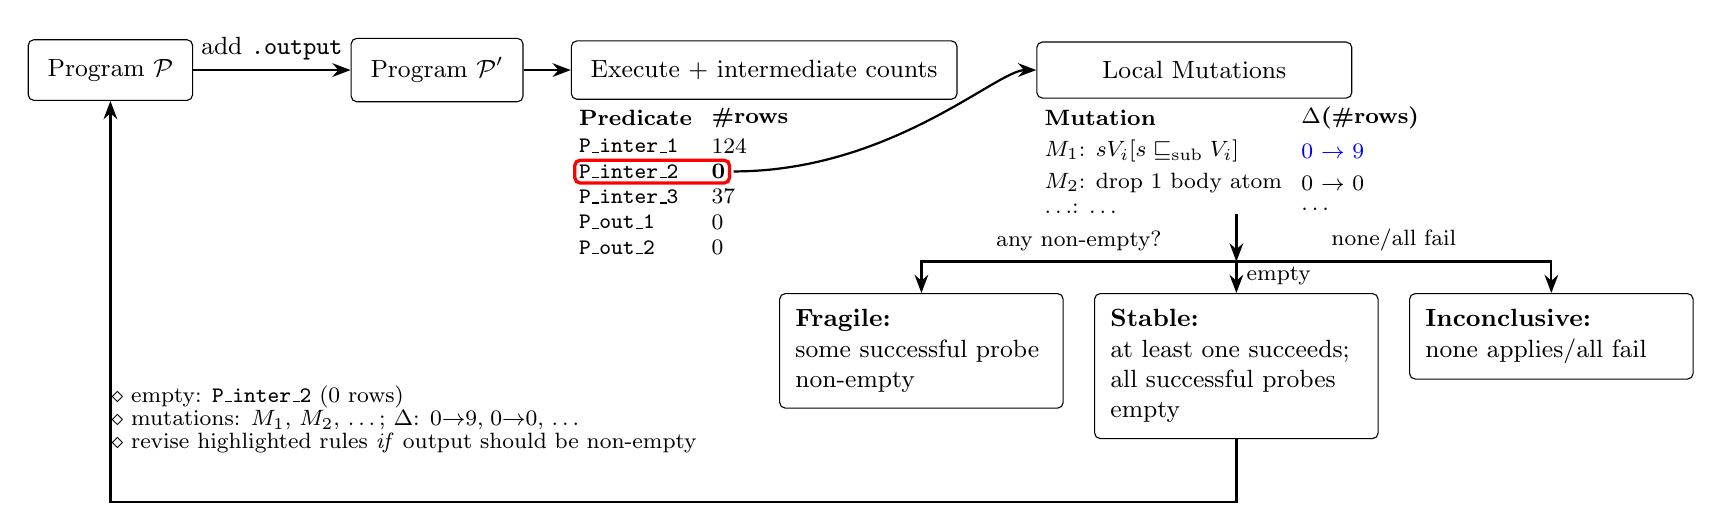
\begin{tikzpicture}[
  font=\small,
  node distance=12mm and 16mm,
  >={Stealth[length=2.2mm]},
  line/.style={-Stealth, thick},
  panel/.style={draw, rounded corners=2pt, inner sep=7pt, align=left},
  header/.style={font=\small\bfseries, text=black!70},
  note/.style={draw, rounded corners=2pt, inner sep=5pt, font=\scriptsize, align=left},
  outcome/.style={text width=3.2cm, draw, rounded corners=2pt, align=left, font=\small,
                  inner xsep=2mm, inner ysep=2mm}
]

% Program
\node[panel] (P) {Program $\mathcal{P}$};
\node[panel, right = 2cm of P] (Pmod) {Program $\mathcal{P'}$};
\draw[line] (P.east) to node [midway, above] {\small add \texttt{.output}} (Pmod.west);

% count rows
\node[panel, right= 0.6cm of Pmod, minimum width=3.2cm] (R) {Execute + intermediate counts};
\matrix[
  matrix of nodes,
  anchor=north west,
  inner sep=0pt,
  row sep=4pt,
  column sep=7pt,
  nodes={font=\footnotesize, anchor=west},
  column 2/.style={anchor=east},
] (Rtbl) at ([xshift=1mm,yshift=-1mm]R.south west) {
  \textbf{Predicate} & \textbf{\#rows} \\
  \texttt{P\_inter\_1} & 124        \\
  \texttt{P\_inter\_2} & \textbf{0} \\
  \texttt{P\_inter\_3} & 37         \\
  \texttt{P\_out\_1}   & 0 \\
  \texttt{P\_out\_2}   & 0 \\
};

% highlight the 0-row
\draw[red, very thick, rounded corners=2pt]
  ($(Rtbl-3-1.north west)+(-0.5mm,0.5mm)$) rectangle
  ($(Rtbl-3-2.south east)+(0.5mm,-0.5mm)$);

\draw[line] (Pmod.east) -- (R.west);

% mutation
\node[panel, right= 1cm of R, minimum width=4cm] (M) {Local Mutations};
\matrix[
  matrix of nodes,
  anchor=north west,
  inner sep=0pt,
  row sep=4pt,
  column sep=7pt,
  nodes={font=\footnotesize, anchor=west},
  column 2/.style={anchor=east},
] (Mtbl) at ([xshift=1mm,yshift=-1mm]M.south west) {
  \textbf{Mutation} & \textbf{$\Delta$(\#rows) } \\
  $M_1$: $s \rightsquigarrow V_i [s\sqsubseteq_{\mathrm{sub}}V_i]$ & \textcolor{blue}{0 $\rightarrow$ 9} \\
  $M_2$: drop 1 body atom &  0 $\rightarrow$ 0\\
  $\ldots$: \ldots &  \ldots \\
};

% arrow from detected empty to mutation
\draw[line] ([xshift=1mm]Rtbl-3-2.east) .. controls ++(2cm,0)
     and ([xshift=-5mm]M.west) .. (M.west);

% decision: classify empty relation
\node[outcome, below=10mm of Mtbl, xshift=-4.0cm] (frag)
{\textbf{Fragile:}\\ some successful probe non-empty};

\node[outcome, below=10mm of Mtbl] (stab)
{\textbf{Stable:}\\ at least one succeeds;\\ all successful probes empty};

\node[outcome, below=10mm of Mtbl, xshift=+4.0cm] (inc)
{\textbf{Inconclusive:}\\ none applies/all fail};

% junction point under Local Mutations
\coordinate (dec) at ([yshift=-6mm]Mtbl.south);
% stem + forks
\draw[line] ([yshift=0mm]Mtbl.south) -- (dec);

\draw[line]
  (dec) -| node[pos=0.25, above, sloped, font=\footnotesize] {any non-empty?}
  (frag.north);

\draw[line]
  (dec) -- node[pos=0.45, right, font=\footnotesize] {empty}
  (stab.north);

\draw[line]
  (dec) -| node[pos=0.25, above, sloped, font=\footnotesize] {none/all fail}
  (inc.north);

% Feedback 

% connect classification to feedback (single clean arrow)
\coordinate (classout) at (stab.south);
\draw[line]
  (classout) -- ++(0,-8mm) -|
  node[
    pos=0.55,
    anchor=south west,
    inner sep=0pt,
    matrix of nodes,
    row sep=1.1pt,
    yshift=1mm,
    nodes={font=\footnotesize, anchor=west, align=left}
  ] (Ftxt) {
    $\diamond$ empty: \texttt{P\_inter\_2} (0 rows) \\
    $\diamond$ mutations: $M_1$, $M_2$, \ldots; $\Delta$: 0$\rightarrow$9,\;0$\rightarrow$0, \ldots \\
    $\diamond$ revise highlighted rules \emph{if} output should be non-empty \\
  }
  (P.south);

\end{tikzpicture}
\end{document}

%%% Local Variables:
%%% mode: LaTeX
%%% TeX-master: t
%%% End:
